\section{Neural SINDy: Sparse ID with Grokked MLP Libraries}

\subsection*{The Task}

SINDy (Sparse Identification of Nonlinear Dynamics) discovers the ODE
governing a time series by picking a sparse combination from a
hand-crafted library of basis functions:
\[
    \dot{X} \;=\; \Theta(X) \cdot \xi, \qquad
    \Theta(X) = [1,\; x,\; x^2,\; \sin x,\; \cos x,\; \ldots]
\]

Standard SINDy needs a human to curate $\Theta$. \emph{Neural SINDy}
replaces each basis function with a small MLP that has \emph{grokked}
one operation --- \texttt{identity}, \texttt{sin}, \texttt{cos},
\texttt{add}, \texttt{mul} --- so the library becomes a learned
component. The sparse regression then selects which learned
\emph{operations} best explain the observed dynamics.

The target is a damped harmonic oscillator with $k=1.0$, $c=0.1$:
\[
    \ddot{x} \;=\; -k\,x - c\,\dot{x}
    \qquad \Longleftrightarrow \qquad
    \dot{x} = v, \;\; \dot{v} = -k\,x - c\,v
\]
600 time points, small Gaussian noise. Success means recovering those
two equations with clean, interpretable coefficients.

\subsection*{Pipeline (Phases 1--3)}

\paragraph{Phase 1.} Train 5 MLPs past overfitting on basic operations
--- AdamW with heavy weight decay for 10k--20k epochs each. Training
loss drops fast; validation loss drops much later (grokking). Each MLP
ends as a clean algorithmic circuit for its target function.

\paragraph{Phase 2.} Simulate the oscillator; collect
$[t, x, v, \dot{x}, \dot{v}]$.

\paragraph{Phase 3.} Build $\Theta(X)$ by passing the state data
through each grokked MLP (8 terms total: \texttt{identity}, \texttt{sin},
\texttt{cos} on $x$ and $v$, plus \texttt{add(x,v)} and
\texttt{mul(x,v)}), then solve for a sparse $\xi$.

\subsection*{Run 1: STLSQ Baseline --- Correct Answer, Ugly Presentation}

Sequential Thresholded Least Squares fits exactly --- MSE $10^{-6}$ ---
but the coefficients are distributed across redundant terms:
\[
    \dot{x} \;\approx\; -0.333\cdot\mathrm{id}(x) +0.667\cdot\mathrm{id}(v) +0.332\cdot\mathrm{add}(x,v)
\]
\[
    \dot{v} \;\approx\; -0.632\cdot\mathrm{id}(x) +0.268\cdot\mathrm{id}(v) -0.368\cdot\mathrm{add}(x,v)
\]

Summing simplifies cleanly to the truth ($\dot{x}=v$,
$\dot{v}=-x-0.1v$), but the individual coefficients are uninterpretable.
The reason is an \emph{exact collinearity} in the library:
$\mathrm{add}(x,v) = \mathrm{id}(x)+\mathrm{id}(v)$, so $\Theta$ is
rank-deficient. STLSQ --- even with ridge regularization --- cannot
distinguish the redundant directions and splits coefficients
arbitrarily. Dropping \texttt{add} from the library is the one-line fix;
a more principled fix would move to a method that doesn't invert $\Theta$
at all.

\textbf{Hypothesis.} A differentiable Gumbel-Softmax router over the
library would pick terms categorically rather than solving a linear
system, sidestepping rank deficiency.

\subsection*{Run 2 (Exp 1): Gumbel-Softmax, Softmax Soup}

\begin{center}
    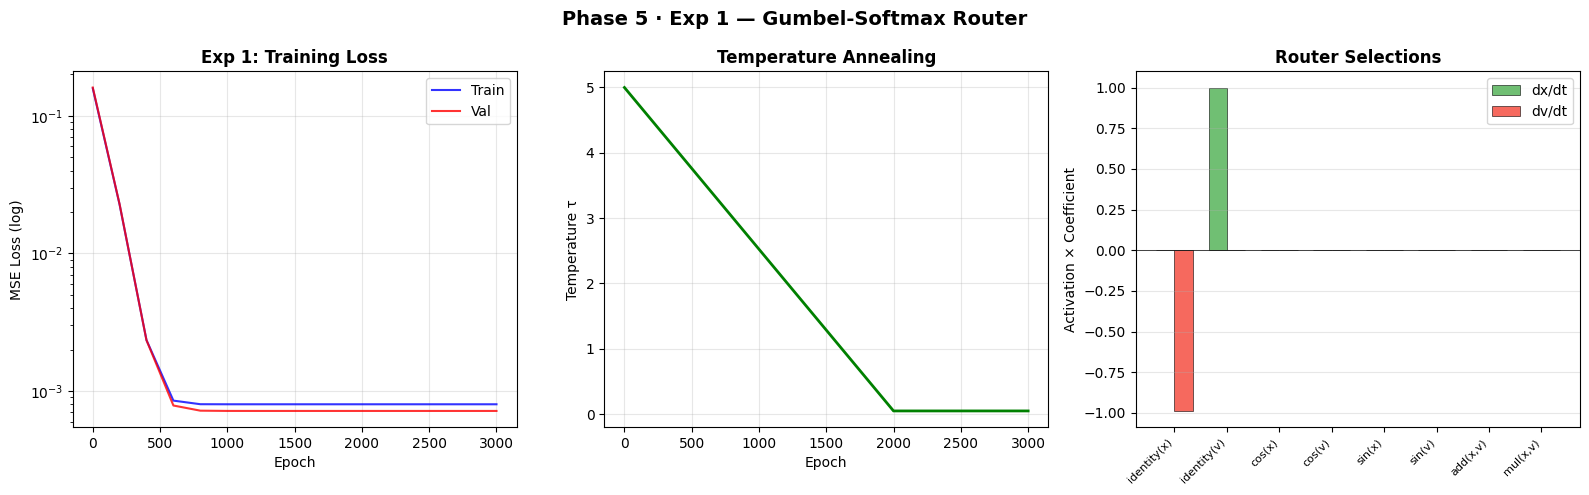
\includegraphics[width=0.9\linewidth]{figures/sindy_exp1_softmax_soup.png}
\end{center}

A state-dependent router (Linear $\to$ ReLU $\to$ Linear $\to$ ReLU
$\to$ Linear) with Gumbel-Softmax sampling and temperature annealing
$\tau: 5.0 \to 0.05$. Expected near-one-hot activations; got a
``softmax soup'' instead.

\begin{center}
    \begin{tabular}{lrr}
        \toprule
        & max activation & final MSE \\
        \midrule
        $\dot{x}$ & $43.8\%$ (\texttt{identity(v)}) & \multirow{2}{*}{$\sim 5 \cdot 10^{-3}$} \\
        $\dot{v}$ & $19.2\%$ (\texttt{identity(x)}) & \\
        \bottomrule
    \end{tabular}
\end{center}

The router found the right dominant term ($\mathrm{id}(v)$ with
coefficient $+1.0000$) but never committed. Three failures stacked:

\paragraph{No sparsity pressure.} Nothing in the loss pushes the logits
apart. With high $\tau$ the router computes a weighted average across
all MLPs and tunes per-MLP coefficients to fit the data. When $\tau$
drops at epoch 2000, the underlying distribution never concentrated,
and the soft-vs-hard mismatch shows as a loss discontinuity.

\paragraph{Damping lost.} $\dot{v}$'s damping term $-0.1\,v$ is
$10\times$ smaller than the restoring force. Without sparsity, that
signal is drowned across 7 other terms.

\paragraph{Collinearity in disguise.} \texttt{add(x,v)} is still
selected 10--14\% of the time with meaningful coefficients. Rank
deficiency didn't disappear --- it became probability-mass splitting.

Net: MSE $\sim 1000\times$ worse than STLSQ. \emph{Gumbel-Softmax
without entropy regularization is just a fancy softmax.}

\subsection*{Run 3 (Exp 2): Scalar Router + Entropy --- Wrong Basis}

\begin{center}
    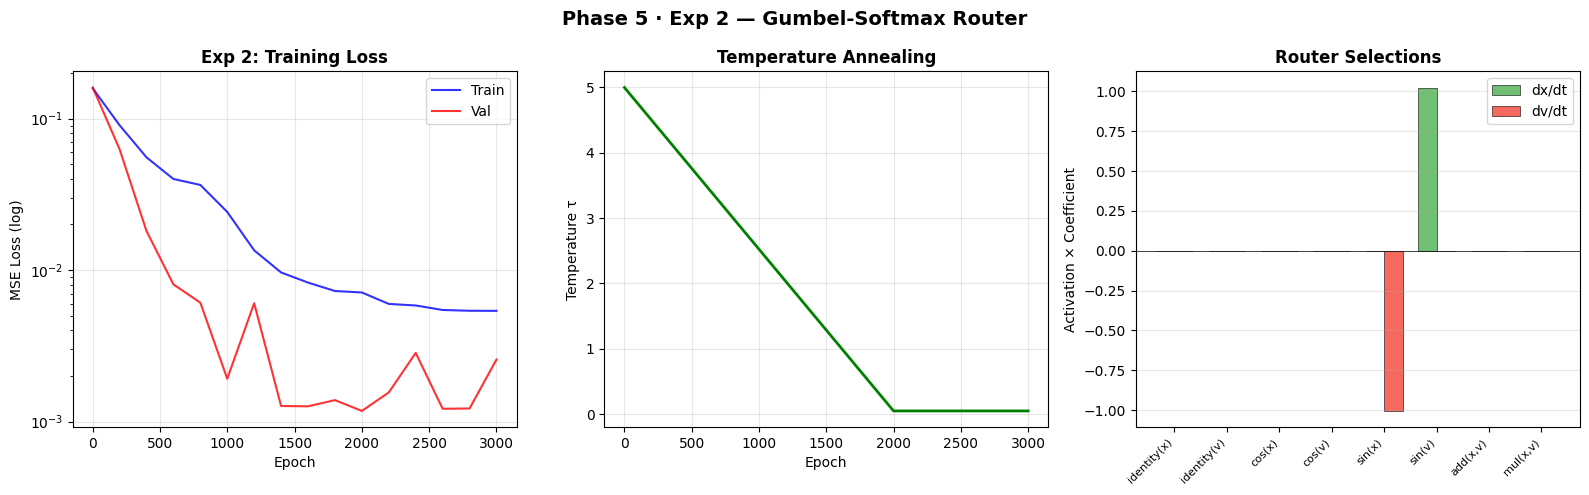
\includegraphics[width=0.9\linewidth]{figures/sindy_exp2_scalar_router.png}
\end{center}

Three changes from Exp 1:
\begin{enumerate}
    \item \textbf{State-independent router.} A single learnable logit
          vector per derivative, broadcast across the batch. Matches
          the SINDy assumption that one term governs the dynamics
          everywhere in state space. Param count drops from
          $9{,}760 \to 32$.
    \item \textbf{Entropy penalty with correct sign, scheduled weight:}
          $w = 0.05 \cdot \max(0, 1 - \tau/\tau_{\text{start}})$. Zero
          at the start (pure exploration); $\sim 0.05$ at the end
          (strong pressure toward one-hot).
    \item Same Gumbel-Softmax + anneal schedule.
\end{enumerate}

Result: clean one-hot commitment.

\begin{center}
    \begin{tabular}{lrr}
        \toprule
        & selected term & activation \\
        \midrule
        $\dot{x}$ & $+1.0265 \cdot \sin(v)$  & $99.7\%$ \\
        $\dot{v}$ & $-1.0138 \cdot \sin(x)$  & $99.2\%$ \\
        \bottomrule
    \end{tabular}
\end{center}

Wrong basis. The true equations are linear in $x, v$, so
$\mathrm{id}(x)$ and $\mathrm{id}(v)$ should have won. The router
picked \texttt{sin} instead because $\sin(z) \approx z$ within $\sim
15\%$ for $|z| \lesssim 1$ (the amplitudes the oscillator visits).
The inflated coefficient ($1.0265$ vs.\ true $1.0$) absorbs the
Taylor-series shortfall. The entropy penalty broke the near-tie
arbitrarily.

Damping is still gone: one-hot \emph{structurally cannot} represent a
two-term equation like $\dot{v} = -1 \cdot x - 0.1 \cdot v$.

\paragraph{Two collinearities, not one.} Exp 1 hit the \emph{exact}
collinearity $\mathrm{add}(x,v) = \mathrm{id}(x) + \mathrm{id}(v)$.
Exp 2 sidesteps that but hits an \emph{approximate} collinearity
$\sin(z) \approx z$. The library design is the real bottleneck; both
optimizers are doing their jobs.

\subsection*{Run 4 (Exp 3): Top-$k$ + Complexity Prior --- Dominant Term Recovered}

\begin{center}
    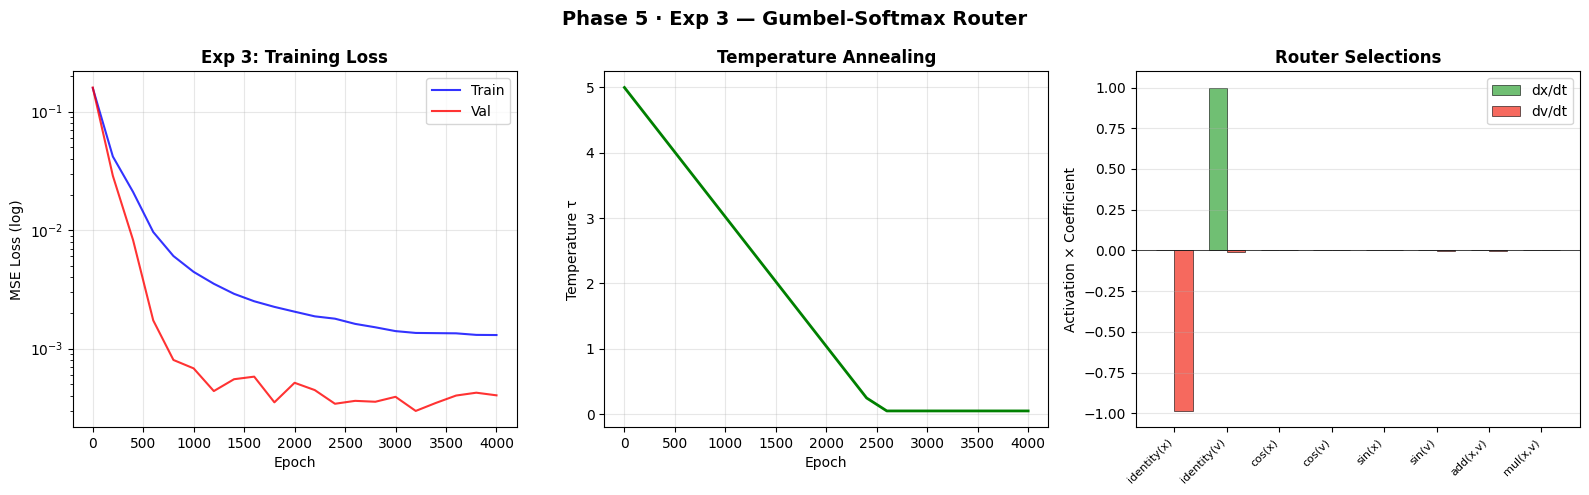
\includegraphics[width=0.9\linewidth]{figures/sindy_exp3_topk_prior.png}
\end{center}

Two changes:

\paragraph{Top-$k$ routing ($k{=}2$).} Each derivative selects two
basis functions instead of one. Implemented as $k$ independent
Gumbel-Softmax draws with prior selections masked out (sampling-
without-replacement via iterative masked argmax with STE gradients).
Each slot has its own learnable coefficient. Now $\dot{v} = -1\cdot x -
0.1\cdot v$ is \emph{representable}.

\paragraph{Complexity prior ($\alpha{=}1.0$).} Occam's razor baked into
the logits: $\mathrm{identity} \prec \sin/\cos \prec$ binary MLPs.
Added directly to the logits so it biases selection without distorting
learned coefficients.

\medskip

Result:
\[
    \dot{x} \;=\; +1.0000 \cdot \mathrm{id}(v)
\]
\[
    \dot{v} \;=\; -0.9853 \cdot \mathrm{id}(x) -0.0267 \cdot \mathrm{id}(v) -0.0151 \cdot \sin(v)
\]

\begin{center}
    \begin{tabular}{lrrr}
        \toprule
        term                   & discovered & true & error \\
        \midrule
        $\mathrm{id}(v)$ in $\dot{x}$ & $+1.0000$ & $+1.0$ & $0.00\%$ \\
        $\mathrm{id}(x)$ in $\dot{v}$ & $-0.9853$ & $-1.0$ & $1.5\%$  \\
        $\mathrm{id}(v)$ in $\dot{v}$ & $-0.0267$ & $-0.1$ & $73\%$   \\
        \bottomrule
    \end{tabular}
\end{center}

Slot 1 locks cleanly on the correct basis in both derivatives. Slot 2
identifies $\mathrm{id}(v)$ as the right damping term but fails to
commit --- selected only 27\% of the time, with a coefficient $\sim
1/4$ the true magnitude.

\subsection*{Run 5 (Exp 4): Conditional Slot Entropy --- Diagnosis}

\begin{center}
    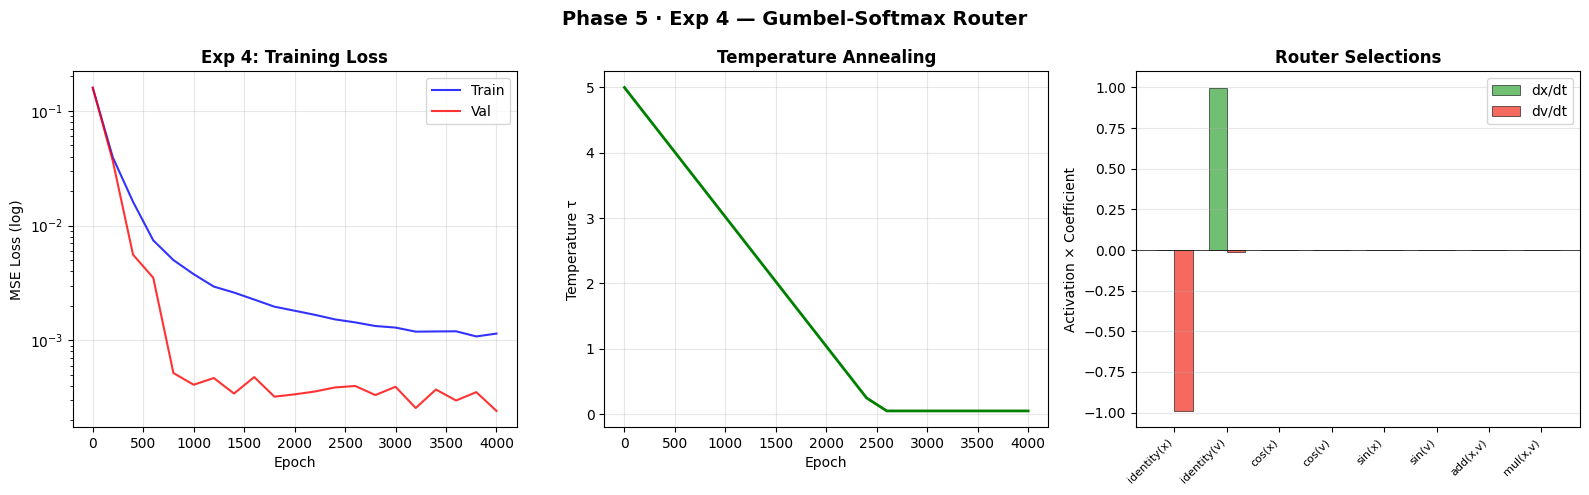
\includegraphics[width=0.9\linewidth]{figures/sindy_exp4_conditional_entropy.png}
\end{center}

\paragraph{Root cause found.} Exp 3's entropy penalty operated on the
\emph{base} distribution $\mathrm{softmax}(\mathrm{logits}+\mathrm{prior})$
--- before any masking. Minimizing that drove the base distribution
one-hot on the dominant term. Once slot 1 committed and masked its
winner to $-\infty$, slot 2 faced a near-flat \emph{conditional}
distribution with no gradient pointing it anywhere useful.

\paragraph{Fix.} Iterate slot-by-slot, mirroring the forward pass:
\[
    H_j = -\!\!\sum \mathrm{softmax}(\mathrm{logits} + \mathrm{mask}_j)
          \cdot \log \mathrm{softmax}(\mathrm{logits} + \mathrm{mask}_j),
    \quad
    \mathrm{mask}_{j+1} \mathrel{+}= -\infty \;\text{at}\; \arg\max_j
\]
Each slot's \emph{conditional} distribution is penalized
independently. Slot 2 now receives a direct gradient to concentrate on
whatever term best explains the residual.

\medskip

Result: slot 1 unchanged (100\% commitment, coefficients unchanged).
Slot 2's $\mathrm{id}(v)$ activation improves from 27\% $\to$ 34\%;
damping coefficient from $-0.027 \to -0.034$. Val MSE $2.42 \cdot
10^{-4}$, still $\sim 24\times$ above the $10^{-5}$ target.

\paragraph{Why slot 2 still won't commit.} Three compounding factors:

\begin{enumerate}
    \item \textbf{Weak residual signal.} After slot 1 absorbs $\sim
          99\%$ of $\dot{v}$ variance, the residual slot 2 must explain
          is $\sim 10\times$ smaller than the primary signal.
          Reconstruction-loss gradient to slot 2 is proportionally weak.
    \item \textbf{STE gradient starvation at low $\tau$.} At $\tau =
          0.05$, the Straight-Through Estimator back-propagates through
          soft weights that are essentially zero for non-winners.
          Slot 2's losing logits barely move.
    \item \textbf{Entropy budget split equally.} The entropy weight
          applies to both slots, but slot 1 is already committed and
          doesn't need pressure. Budget wasted.
\end{enumerate}

\subsection*{Summary of Runs}

\begin{center}
    \begin{tabular}{clrrc}
        \toprule
        Run & Method                        & Val MSE           & Max act. & Correct? \\
        \midrule
        1   & STLSQ                         & $10^{-6}$         & ---      & structure: yes; coeffs: spread \\
        2   & Gumbel, MLP router            & $\sim 5\cdot 10^{-3}$ & $44\%$   & soft mixture, damping gone \\
        3   & Gumbel, scalar + entropy      & $\sim 1\cdot 10^{-3}$ & $99.7\%$ & wrong basis (\texttt{sin} vs id) \\
        4   & + top-$k$ + complexity prior  & $\sim 3\cdot 10^{-4}$ & $100\%$  & right basis; damping at $27\%$ \\
        5   & + conditional slot entropy    & $2.4\cdot 10^{-4}$ & $100\%$  & damping at $34\%$ \\
        \bottomrule
    \end{tabular}
\end{center}

\subsection*{What I Learned}

Each failure revealed something different about the library-vs-optimizer
interplay:

\begin{enumerate}
    \item STLSQ fails on \emph{exact} collinearity because it inverts a
          rank-deficient $\Theta$; it distributes coefficients rather
          than picking.
    \item Gumbel-Softmax without an entropy penalty stays soft.
          Categorical sampling doesn't imply categorical commitment;
          the loss has to ask for it.
    \item One-hot with entropy cannot represent multi-term equations
          and picks arbitrarily among \emph{approximately} collinear
          terms ($\sin \approx \mathrm{id}$ for small amplitudes).
    \item Top-$k$ + complexity prior fixes both, but the joint loss
          starves slot 2's gradient when the residual signal is $10\times$
          smaller than the primary term.
\end{enumerate}

The library has two collinearities --- one exact, one approximate ---
and every method ``failed'' by exposing one of them. The real fix
lives upstream of the router: drop \texttt{add} from the library, train
slot 2 on an explicit residual
$\dot{v} - \xi_1 \cdot \mathrm{basis}_1(X)$, or freeze slot 1 after
commitment and fine-tune slot 2 alone. All three give the weak damping
term a full-strength gradient instead of a fraction of the joint loss.

The template, again: when a method fails, the failure mode is usually
more informative than the failure magnitude. STLSQ's MSE of $10^{-6}$
looked like success and was hiding a rank-deficient library; the
router's MSE of $5\cdot 10^{-3}$ looked like failure and pointed
directly at the missing sparsity objective. Reading the residuals ---
\emph{per term}, not in aggregate --- is where the signal lives.
